\subsection{Person 4 – SUS 70}  
\textbf{Zur Person:}\\
Medizin-Studentin, 24 Jahre alt 

\textbf{Beobachtung:}  
\begin{enumerate}
    \item Zeichnen Sie frei für etwa 2 Minuten.
    \begin{itemize}
        \item Pen-Einstellungen nicht klar.
        \item PDF-Control-Icons nicht intuitiv.
        \item Undo-Button fehlt.
    \end{itemize}

    \item Löschen Sie Ihre Zeichnung vollständig.
    \begin{itemize}
        \item Kein intuitiver Button vorhanden.
    \end{itemize}

    \item Laden Sie die PDF-Datei mit dem Grundriss hoch.
    \begin{itemize}
        \item Keine Probleme.
    \end{itemize}

    \item Ändern Sie die Stiftfarbe auf Rot.
    \begin{itemize}
        \item Klar nach Aufgabenstellung, keine Probleme.
    \end{itemize}

    \item Suchen Sie \texttt{BEDROOM3} und zeichnen Sie einen Tisch links vom Bett.
    \begin{itemize}
        \item Keine Probleme.
    \end{itemize}

    \item Radieren Sie den Tisch und zeichnen Sie ihn rechts vom Bett.
    \begin{itemize}
        \item Am Anfang Zickzack-Bug, danach keine Probleme.
    \end{itemize}

    \item Zeichnen Sie die Abmessungen 1\,m $\times$ 1\,m und schreiben Sie «table» hinein.
    \begin{itemize}
        \item Keine Probleme.
    \end{itemize}

    \item Speichern Sie den Plan auf Ihrem Laptop.
    \begin{itemize}
        \item Keine Probleme.
    \end{itemize}
\end{enumerate}

\clearpage

\textbf{SUS-Antworten (Bild):}
\begin{center}
    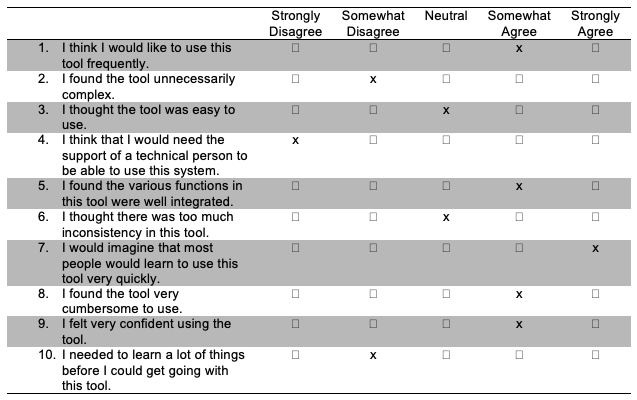
\includegraphics[width=0.95\textwidth]{graphics/sus_person4.png}
\end{center}

\textbf{Follow-up:}  
\begin{enumerate}
    \item \textbf{Was hat Ihnen am Tool am besten gefallen?}
    \begin{itemize}
        \item Dateihandling einfach zu bedienen, ohne viel Klicken.
    \end{itemize}

    \item \textbf{Gab es etwas, das verwirrend oder schwierig zu bedienen war?}
    \begin{itemize}
        \item Zickzack-Bug beim Zeichnen.
        \item Undo-Button fehlt.
    \end{itemize}

    \item \textbf{Fehlt etwas, das Sie erwartet oder gerne gehabt hätten?}
    \begin{itemize}
        \item Undo-Button.
        \item Finger-Touch-Support.
        \item Drei Modi, um das Dokument zu verschieben; aktuelle Buttons umständlich.
    \end{itemize}

    \item \textbf{Haben Sie Vorschläge, wie das Tool verbessert werden könnte?}
    \begin{itemize}
        \item „Premium Feature“: automatische Formgenerierung (z.B. Quadrat 1\,m x 1\,m in Fläche ziehen).
        \item Verschieben von Zeichnungen.
        \item Hintergrund sollte nicht mit Radiert werden – aktuell unintuitiv.
    \end{itemize}
\end{enumerate}

\clearpage
